\documentclass{article} % lub inna klasa dokumentu, np. report lub book
\usepackage[utf8]{inputenc} % ustawienie kodowania na UTF-8
\usepackage{amsmath, amssymb, amsthm} % biblioteki do działań matematycznych
\usepackage[T1]{fontenc}    % wybór odpowiedniego kodowania czcionek
\usepackage{polski}         % dodanie wsparcia dla polskich znaków
\usepackage{babel}          % automatyczne dostosowanie języka
\usepackage{pgfplots}       % Pakiet do tworzenia wykresów
\usepackage{verbatim}
\pgfplotsset{compat=1.18}

\title{Sprawozdanie}

\author{Tomasz Lisowski 197749\and Filip Świniarski 197725\and Nikodem Miłuch 197922}


\begin{document}
\maketitle

\section{Wstęp}

Celem ćwiczenia jest pomiar oporu elektrycznego pojedynczych rezystorów
oraz układu rezystorów połączonych szeregowo z wykorzystaniem mostka prądu stałego (mostek Wheatstone’a).

\subsection{Mostek Wheatstone'a}

Mostek Wheatstone’a to precyzyjny układ elektryczny służący do pomiaru nieznanych wartości rezystancji. Składa się z czterech rezystorów połączonych w formie mostka, do którego podłączone są źródło napięcia oraz galwanometr umożliwiający wykrywanie równowagi mostka. Mostek jest w równowadze, gdy prąd płynący przez galwanometr wynosi zero. Dzieje się tak, gdy stosunek rezystancji w jednej gałęzi równa się stosunkowi rezystancji w drugiej gałęzi.

\section{Wyznaczenie rezystancji wybranych rezystorów}

\subsection{Opis doświadczenia}

Do płytki wchodzącej w skład zestawu doświadczalnego zostały szeregowo wpięte dwa rezystory. Pomiar rezystancji drugiego opornika przebiegał następująco:
{\begin{enumerate}
    \item Szeregowe połączenie wybranych rezystorów.
    \item Zasilenie układu prądem $I = 1A$ oraz $U = 0.65V$.
    \item Pomiar stosunku długości dwóch części potencjometru.
\end{enumerate}
}

\subsection{Wyprowadzenie wzorów}

Korzystając ze wzorów prawdziwych dla układu mostka Wheatstone'a otrzymujemy:
{\large
\begin{equation}
    R_x = R_n\frac{l_1}{l_2}
\end{equation}}

Gdzie: $R_x$ - szukana rezystancja, $R_n$ - opór znanego rezystora, $l_1, l_2$ - długości przewodników. Należy zauważyć, że $l_1 + l_2 = L$. $L$ jest długością całego przewodnika, na którym zbudowany jest potencjometr.

\subsection{Niepewność pomiarowa}

Niepewność pomiarową wyznaczamy jako niepewność wielkość złożonej. Błąd pomiarowy pomiaru długości $l_1, l_2$ wyznaczamy na podstawie podziałki potencjometru. W tym przypadku $\Delta l$ = 0.001[m]. Pochodne cząstkowe mierzonych wartości ze wzoru (1) przyjmują wartości:
{\large
\begin{equation}
\frac{\partial R_x}{\partial l_1} = R_n\frac{1}{l_2}    
\end{equation}
}

{\large
\begin{equation}
\frac{\partial R_x}{\partial l_2} = R_n\frac{l_1}{l_2^2}    
\end{equation}
}
Ostatecznie:
{\large
\begin{equation}
\Delta R_x = \sqrt{(R_n\frac{\Delta l}{l_2} )^2+(R_n\frac{l_1\Delta l}{l_2^2})^2}   
\end{equation}
}
\subsection{Wyniki pomiarów}

Dane pomiarowe zebrano w Tabeli 1.
\begin{table}[h!]
\centering
\begin{tabular}{|c|c|c|}
\hline
\textbf{Rezystor} & \textbf{$l_2$[m]} & \textbf{$l_1$[m]} \\
\hline
 2 & 0.124 & 0.876 \\
 5 & 0.410 & 0.590 \\
\hline
\end{tabular}
\caption{Wyniki pomiarów}
\label{table:students}
\end{table}

\subsection{Wyniki doświadczenia}

Ostateczny wynik rezystancji oporników 2 i 5 otrzymujemy poprzez podstawienie odpowiednich danych do wzorów (1) i (4). Wyniki zebrano w Tabeli 2.

\begin{table}[h!]
\centering
\begin{tabular}{|c|c|}
\hline
\textbf{Rezystor} & \textbf{Opór[$\Omega$]} \\
\hline
 2 & 0.142 \\
 5 & 0.695 \\
\hline
\end{tabular}
\caption{Wyniki doświadczenia}
\label{table:students}
\end{table}
W obu przypadkach błąd pomiarowy był zbliżony do $\Delta l$ i wynosił $\Delta R_x$ = 0.0015$\Omega$

\section{Szeregowy układ rezystorów}

\subsection{Opis doświadczenia}

Przebieg doświadczenie wygląda identycznie jak w punkcie 2. Jedyna istotna zmiana to przepięcie rezystorów na płytce w taki sposób, aby stworzyły układ szeregowy.

\subsection{Wyniki pomiarów}

Wyniki pomiarów szeregowego układu rezystorów przedstawiono w Tabeli 3.

\begin{table}[h!]
\centering
\begin{tabular}{|c|c|c|}
\hline
\textbf{Rezystor} & \textbf{$l_2$[m]} & \textbf{$l_1$[m]} \\
\hline
 Układ (2+5) & 0.460 & 0.540 \\
\hline
\end{tabular}
\caption{Wyniki pomiaru szeregowego układu rezystorów}
\label{table:students}
\end{table}

\subsection{Wyniki doświadczenia}
Podstawiając dane z Tabeli 3 do wzorów (1) i (4) otrzymujemy:
{\large
\begin{equation}
    R_{sz} = 0.851\pm0.002\Omega
\end{equation}
}
Matematyczne wyznaczenie układu daje podobny wynik wynoszący:
{\large
\begin{equation}
    R_{sz} = 0.837\pm0.002\Omega
\end{equation}
}


\section{Równoległy układ rezystorów}


\subsection{Opis doświadczenia}

Przebieg doświadczenie wygląda identycznie jak w punkcie 2. Jedyna istotna zmiana to przepięcie rezystorów na płytce w taki sposób, aby stworzyły układ równoległy.

\subsection{Wyniki pomiarów}

Wyniki pomiarów równoległego układu rezystorów przedstawiono w Tabeli 4.

\begin{table}[h!]
\centering
\begin{tabular}{|c|c|c|}
\hline
\textbf{Rezystor} & \textbf{$l_2$[m]} & \textbf{$l_1$[m]} \\
\hline
 Układ ($\frac{1}{2}+\frac{1}{5}$) & 0.104 & 0.894 \\
\hline
\end{tabular}
\caption{Wyniki pomiaru równoległego układu rezystorów}
\label{table:students}
\end{table}

\subsection{Wyniki doświadczenia}
Podstawiając dane z Tabeli 4 do wzorów (1) i (4) otrzymujemy:
{\large
\begin{equation}
    R_{rw} = 0.116\pm0.001\Omega
\end{equation}
}
Matematyczne wyznaczenie układu daje podobny wynik wynoszący:
{\large
\begin{equation}
    R_{rw} = 0.101\pm0.001\Omega
\end{equation}
}
\section{Przewody konstantanowe}

\subsection{Opis doświadczenia}

W ramach sprzętu laboratoryjnego udostępnione zostały 4 druty zrobione z konstantanu. Poprzez wpinanie ich w układ, w którym płynął prąd o stałym napięciu i natężeniu oraz wykorzystanie miernika dekadowego można wyznaczyć zależność oporu od średnicy.

\subsection{Wyprowadzenie wzorów}

Oby wykreślić zależność oporu elektrycznego od posłużymy się wzorem na na opór właściwy:
{\large
\begin{equation}
    R_w = \rho\frac{l}{S}
\end{equation}
}
gdzie $\rho$ - opór właściwy, a $l, S$ to kolejno długość i pole przekroju przewodnika. Ponieważ dane doświadczalne to $R_w$ opór elektryczny oraz $d$ - średnia przewodu wzór (9) przyjmuje postać:
{\large
\begin{equation}
    R_w = \rho\frac{4l}{\pi d^2}
\end{equation}
}
Ponieważ człon $\rho\frac{4l}{\pi}$ jest stały dla każdego pomiaru, wykres $f(\frac{1}{d^2})$ będzie miał charakter liniowy.
\subsection{Niepewność pomiarowa}

Niepewność pomiaru to $\Delta r$ = 0.1[$\Omega$].
Ostatecznie niepewność pomiarowa dana jest wzorem:

\subsection{Wyniki doświadczenia}

\begin{center}
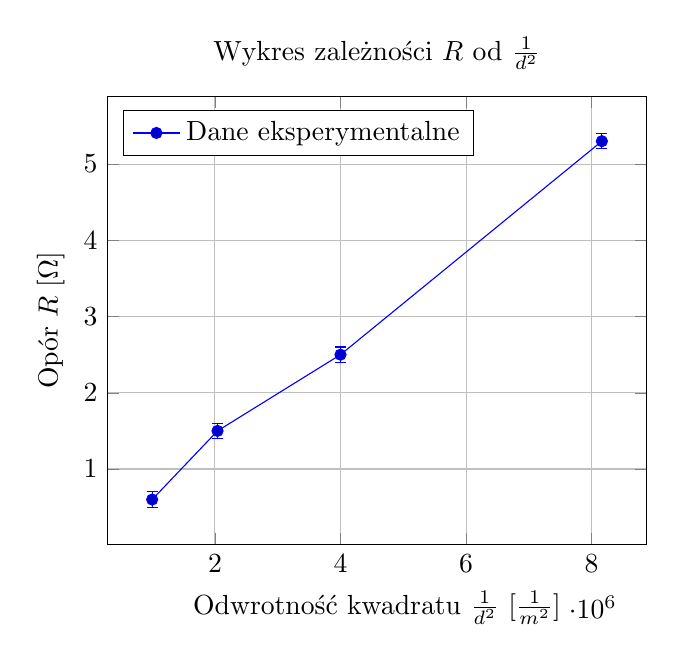
\begin{tikzpicture}
    \begin{axis}[
        ylabel={Opór $R$ [$\Omega$]}, % Etykieta osi X
        xlabel={Odwrotność kwadratu  $\frac{1}{d^2}$ [$\frac{1}{m^2}$]},             % Etykieta osi Y
        grid=major,                        % Siatka na wykresie
        legend pos=north west,             % Pozycja legendy
        title={Wykres zależności $R$ od $\frac{1}{d^2}$}, % Tytuł wykresu
    ]
    \addplot+[
        mark=*,
        color=blue,
        error bars/.cd,
        y dir=both, % Enable error bars in both upward and downward directions
        y explicit % Explicitly define the errors
    ] coordinates {
        (8163265, 5.3) +- (0,0.1)
        (4000000, 2.5) +- (0,0.1)
        (2040816.33, 1.5) +- (0,0.1)
        (1000000, 0.6) +- (0,0.1)
        
    };
    \addlegendentry{Dane eksperymentalne}
    \end{axis}
\end{tikzpicture}
\end{center}
Podstawiając odpowiednie dane do wzoru (10) otrzymujemy teoretyczny współczynnik kierunkowy. Dla $\rho = 0.5 \cdot10^{-6}$ $\Omega \cdot m$, oraz $l = 1$ m. Jego wartość wynosi:
{\large
\begin{equation}
    a = 0.63 \quad \Omega \cdot m^2
\end{equation}
}
Uśredniając dane z wykresu otrzymujemy wynik:
{\large
\begin{equation}
    a = 0.67 \quad \Omega \cdot m^2
\end{equation}
}
Wyniki są do siebie zbliżone.
\section{Opór właściwy konstantanu}
\subsection{Wyznaczenie wzorów}
Przekształcając wzór (10) otrzymujemy wzór na opór właściwy:
{\large
\begin{equation}
    \rho = R_w\frac{\pi d^2}{4l}
\end{equation}
}
\subsection{Niepewność pomiarowa}
Jedyną wartością mierzoną w równaniu (13) jest $R_w$ zatem niepewność pomiarowa jest niepewnością złożoną tylko tej wielkości. $\Delta R_w = 0.1$ $\Omega$ Pochodna cząstkowa względem $R_w$ dana jest wzorem:
{\large
\begin{equation}
    \frac{\partial \rho}{\partial R_w} = \frac{\pi d^2}{4l}
\end{equation}
}
Ostateczna niepewność:
{\large
\begin{equation}
    u(f) =  |\frac{\pi d^2}{4l}|\Delta R_w
\end{equation}
}
\subsection{Wyniki doświadczenia}

Korzystając z współczynnika $a$ wyznaczonego metodą graficzną w podpunkcie 5.4 i podstawiając odpowiednie dane do wzorów (13) i (15) otrzymujemy opór właściwy konstantanu równy:
{\large
\begin{equation}
    \rho_k =  0.53 \pm 0.4 \quad\Omega \cdot m
\end{equation}
}
\subsection{Wnioski}
Ostateczny opór właściwy mieści się w przedziale wyznaczonego doświadczalnie oporu właściwego.
\end{document}
